\documentclass[11pt]{article}

\textwidth 16cm \textheight 23cm \evensidemargin 0cm
\oddsidemargin 0cm \topmargin -2cm
\parindent 0pt
\parskip \medskipamount


\usepackage[dutch]{babel}
\usepackage{amssymb}
\usepackage{amsmath}
\usepackage[utf8]{inputenc}
\usepackage[normalem]{ulem} % strikethrough normal text with \sout{text}
\usepackage{cancel} % strikethrough in math mode with \cancel{text}
\usepackage{graphicx}
\usepackage{pgf,tikz}
\usetikzlibrary{arrows}

\usepackage{color}
\newcommand{\todo}[1]{\textcolor{red}{\textbf{\#TODO:} #1\#}}

\newtheorem{onderzoeksvraag}{Onderzoeksvraag}

\begin{document}

\section{Tessellaties van Escher}

\begin{onderzoeksvraag}
Bepaalde kunstwerken van {\it Escher} vullen een vlak met één figuur, waarbij de figuur wordt getransleerd en eventueel geroteerd. Bestaat er een methode om zelf een figuur te ontwerpen die een vlak zo kan vullen?
\end{onderzoeksvraag}

Een voorbeeld van een kunstwerk van Escher waarbij een vlak wordt gevuld met vliegende vissen staat in Figuur \ref{fig:E73}. Deze prent komt uit een reeks van sketchboeken, {\it Regular Division of the Plane Drawings}, die Escher had aangelegd als een bron van ideeën om patronen te kunnen gebruiken in zijn afgewerkte kunstwerken. In het totaal zijn 137 gelijkaardige vlakvullingen te vinden in de sketchboeken.

\begin{figure}[ht]
  \centering
  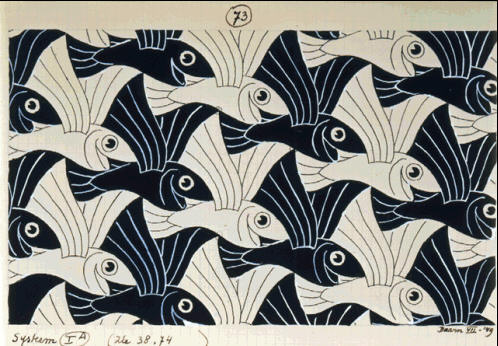
\includegraphics{E73}
  \label{fig:E73}
  \caption{Sketch 73 uit {\it Regular Division of the Plane}.}
\end{figure}


\end{document}























